

\documentclass{beamer}
 
\usepackage[utf8]{inputenc}
 \usetheme{Madrid}
 \usecolortheme{beaver}
 \usefonttheme{structuresmallcapsserif}
 \usepackage{listings}
%Information to be included in the title page:


\title[Distributed Systems] %optional
{Introduction to Distributed systems}

\subtitle{An Overview}

\author[Dr. Joseph Kehoe] % (optional, for multiple authors)
{Joseph Kehoe\inst{1}}

\institute[IT Carlow] % (optional)
{
	\inst{1}%
	Department of Computing and Networking\\
	Institute of Technology Carlow
}

\date[ITC 2018] % (optional)
{CDD101, 2018}

\logo{
\includegraphics[height=1.5cm]{../../itcarlowlogo.png}}




 
 \AtBeginSection[]
 {
 	\begin{frame}
 		\frametitle{Table of Contents}
 		\tableofcontents[currentsection]
 	\end{frame}
 }
 
 
 
\begin{document}
 
\frame{\titlepage}
 
 
 
 \begin{frame}
 	\frametitle{Table of Contents}
 	\tableofcontents
 \end{frame}
 
 
 \section{Definition}
 

  \begin{frame}
  	\frametitle{Definition}
  	\begin{description}
  		\item[Distributed System] A distributed system is a collection of independent computers that appears to its users as a single coherent system
  	\end{description}
  \end{frame}

\section{Why use them?}
  \begin{frame}
  	\frametitle{Why use them?}
  	\begin{description}
  		\item[Distributed System] A distributed system is a collection of independent computers that appears to its users as a single coherent system
  	\end{description}
  \end{frame}
\section{Examples}
  \begin{frame}
  	\frametitle{The Web}
  	\begin{description}
  		\item[Distributed System] A distributed system is a collection of independent computers that appears to its users as a single coherent system
  	\end{description}
  \end{frame}
    \begin{frame}
    	\frametitle{Supercomputers}
    	\begin{description}
    		\item[Distributed System] A distributed system is a collection of independent computers that appears to its users as a single coherent system
    	\end{description}
    \end{frame}
\section{Issues}
  \begin{frame}
  	\frametitle{Issues}
  	\begin{description}
  		\item[Distributed System] A distributed system is a collection of independent computers that appears to its users as a single coherent system
  	\end{description}
  \end{frame}
\section{Next}
  \begin{frame}
  	\frametitle{Early Interfaces}
  	\begin{itemize}
  		\item Input via Punch card
  		\item Output via Line Printer or (small) monochrome screen (or even LEDs)
  	\end{itemize}
  	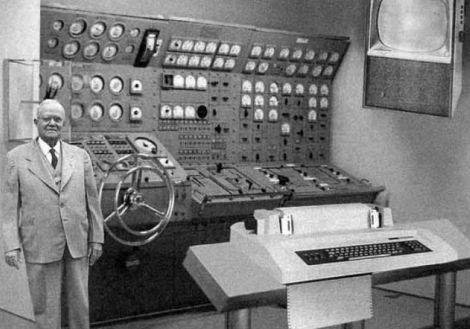
\includegraphics[height=4cm]{Old-Server.jpg}
  	
  \end{frame}
\end{document}

